% Options for packages loaded elsewhere
\PassOptionsToPackage{unicode}{hyperref}
\PassOptionsToPackage{hyphens}{url}
\PassOptionsToPackage{dvipsnames,svgnames,x11names}{xcolor}
%
\documentclass[
]{article}
\title{Modern Data Mining, HW 3}
\author{Group Member Annie Vo \and Group Member Jessica Brown \and Group
Member Sarah Hayward}
\date{Due: 11:59Pm, 2/27, 2022}

\usepackage{amsmath,amssymb}
\usepackage{lmodern}
\usepackage{iftex}
\ifPDFTeX
  \usepackage[T1]{fontenc}
  \usepackage[utf8]{inputenc}
  \usepackage{textcomp} % provide euro and other symbols
\else % if luatex or xetex
  \usepackage{unicode-math}
  \defaultfontfeatures{Scale=MatchLowercase}
  \defaultfontfeatures[\rmfamily]{Ligatures=TeX,Scale=1}
\fi
% Use upquote if available, for straight quotes in verbatim environments
\IfFileExists{upquote.sty}{\usepackage{upquote}}{}
\IfFileExists{microtype.sty}{% use microtype if available
  \usepackage[]{microtype}
  \UseMicrotypeSet[protrusion]{basicmath} % disable protrusion for tt fonts
}{}
\makeatletter
\@ifundefined{KOMAClassName}{% if non-KOMA class
  \IfFileExists{parskip.sty}{%
    \usepackage{parskip}
  }{% else
    \setlength{\parindent}{0pt}
    \setlength{\parskip}{6pt plus 2pt minus 1pt}}
}{% if KOMA class
  \KOMAoptions{parskip=half}}
\makeatother
\usepackage{xcolor}
\IfFileExists{xurl.sty}{\usepackage{xurl}}{} % add URL line breaks if available
\IfFileExists{bookmark.sty}{\usepackage{bookmark}}{\usepackage{hyperref}}
\hypersetup{
  pdftitle={Modern Data Mining, HW 3},
  pdfauthor={Group Member Annie Vo; Group Member Jessica Brown; Group Member Sarah Hayward},
  colorlinks=true,
  linkcolor={Maroon},
  filecolor={Maroon},
  citecolor={Blue},
  urlcolor={blue},
  pdfcreator={LaTeX via pandoc}}
\urlstyle{same} % disable monospaced font for URLs
\usepackage[margin=1in]{geometry}
\usepackage{color}
\usepackage{fancyvrb}
\newcommand{\VerbBar}{|}
\newcommand{\VERB}{\Verb[commandchars=\\\{\}]}
\DefineVerbatimEnvironment{Highlighting}{Verbatim}{commandchars=\\\{\}}
% Add ',fontsize=\small' for more characters per line
\usepackage{framed}
\definecolor{shadecolor}{RGB}{248,248,248}
\newenvironment{Shaded}{\begin{snugshade}}{\end{snugshade}}
\newcommand{\AlertTok}[1]{\textcolor[rgb]{0.94,0.16,0.16}{#1}}
\newcommand{\AnnotationTok}[1]{\textcolor[rgb]{0.56,0.35,0.01}{\textbf{\textit{#1}}}}
\newcommand{\AttributeTok}[1]{\textcolor[rgb]{0.77,0.63,0.00}{#1}}
\newcommand{\BaseNTok}[1]{\textcolor[rgb]{0.00,0.00,0.81}{#1}}
\newcommand{\BuiltInTok}[1]{#1}
\newcommand{\CharTok}[1]{\textcolor[rgb]{0.31,0.60,0.02}{#1}}
\newcommand{\CommentTok}[1]{\textcolor[rgb]{0.56,0.35,0.01}{\textit{#1}}}
\newcommand{\CommentVarTok}[1]{\textcolor[rgb]{0.56,0.35,0.01}{\textbf{\textit{#1}}}}
\newcommand{\ConstantTok}[1]{\textcolor[rgb]{0.00,0.00,0.00}{#1}}
\newcommand{\ControlFlowTok}[1]{\textcolor[rgb]{0.13,0.29,0.53}{\textbf{#1}}}
\newcommand{\DataTypeTok}[1]{\textcolor[rgb]{0.13,0.29,0.53}{#1}}
\newcommand{\DecValTok}[1]{\textcolor[rgb]{0.00,0.00,0.81}{#1}}
\newcommand{\DocumentationTok}[1]{\textcolor[rgb]{0.56,0.35,0.01}{\textbf{\textit{#1}}}}
\newcommand{\ErrorTok}[1]{\textcolor[rgb]{0.64,0.00,0.00}{\textbf{#1}}}
\newcommand{\ExtensionTok}[1]{#1}
\newcommand{\FloatTok}[1]{\textcolor[rgb]{0.00,0.00,0.81}{#1}}
\newcommand{\FunctionTok}[1]{\textcolor[rgb]{0.00,0.00,0.00}{#1}}
\newcommand{\ImportTok}[1]{#1}
\newcommand{\InformationTok}[1]{\textcolor[rgb]{0.56,0.35,0.01}{\textbf{\textit{#1}}}}
\newcommand{\KeywordTok}[1]{\textcolor[rgb]{0.13,0.29,0.53}{\textbf{#1}}}
\newcommand{\NormalTok}[1]{#1}
\newcommand{\OperatorTok}[1]{\textcolor[rgb]{0.81,0.36,0.00}{\textbf{#1}}}
\newcommand{\OtherTok}[1]{\textcolor[rgb]{0.56,0.35,0.01}{#1}}
\newcommand{\PreprocessorTok}[1]{\textcolor[rgb]{0.56,0.35,0.01}{\textit{#1}}}
\newcommand{\RegionMarkerTok}[1]{#1}
\newcommand{\SpecialCharTok}[1]{\textcolor[rgb]{0.00,0.00,0.00}{#1}}
\newcommand{\SpecialStringTok}[1]{\textcolor[rgb]{0.31,0.60,0.02}{#1}}
\newcommand{\StringTok}[1]{\textcolor[rgb]{0.31,0.60,0.02}{#1}}
\newcommand{\VariableTok}[1]{\textcolor[rgb]{0.00,0.00,0.00}{#1}}
\newcommand{\VerbatimStringTok}[1]{\textcolor[rgb]{0.31,0.60,0.02}{#1}}
\newcommand{\WarningTok}[1]{\textcolor[rgb]{0.56,0.35,0.01}{\textbf{\textit{#1}}}}
\usepackage{graphicx}
\makeatletter
\def\maxwidth{\ifdim\Gin@nat@width>\linewidth\linewidth\else\Gin@nat@width\fi}
\def\maxheight{\ifdim\Gin@nat@height>\textheight\textheight\else\Gin@nat@height\fi}
\makeatother
% Scale images if necessary, so that they will not overflow the page
% margins by default, and it is still possible to overwrite the defaults
% using explicit options in \includegraphics[width, height, ...]{}
\setkeys{Gin}{width=\maxwidth,height=\maxheight,keepaspectratio}
% Set default figure placement to htbp
\makeatletter
\def\fps@figure{htbp}
\makeatother
\setlength{\emergencystretch}{3em} % prevent overfull lines
\providecommand{\tightlist}{%
  \setlength{\itemsep}{0pt}\setlength{\parskip}{0pt}}
\setcounter{secnumdepth}{5}
\ifLuaTeX
  \usepackage{selnolig}  % disable illegal ligatures
\fi

\begin{document}
\maketitle

{
\hypersetup{linkcolor=}
\setcounter{tocdepth}{4}
\tableofcontents
}
\pagebreak

\hypertarget{overview}{%
\section{Overview}\label{overview}}

Multiple regression is one of the most popular methods used in
statistics as well as in machine learning. We use linear models as a
working model for its simplicity and interpretability. It is important
that we use domain knowledge as much as we could to determine the form
of the response as well as the function format for the factors. Then,
when we have many possible features to be included in the working model
it is inevitable that we need to choose a best possible model with a
sensible criterion. \texttt{Cp}, \texttt{BIC} and regularizations such
as LASSO are introduced. Be aware that if a model selection is done
formally or informally, the inferences obtained with the final
\texttt{lm()} fit may not be valid. Some adjustment will be needed. This
last step is beyond the scope of this class. Check the current research
line that Linda and collaborators are working on.

This homework consists of two parts: the first one is an excercise (you
will feel it being a toy example after the covid case study) to get
familiar with model selection skills such as, \texttt{Cp} and
\texttt{BIC}. The main job is a rather involved case study about
devastating covid19 pandemic. Please read through the case study first.
It is time that group members work together to run a real project. This
project is for sure a great one listed in your CV.

For covid case study, the major time and effort would be needed in EDA
portion.

\hypertarget{objectives}{%
\subsection{Objectives}\label{objectives}}

\begin{itemize}
\item
  Model building process
\item
  Methods

  \begin{itemize}
  \tightlist
  \item
    Model selection

    \begin{itemize}
    \tightlist
    \item
      All subsets
    \item
      Forward/Backward
    \end{itemize}
  \item
    Regularization

    \begin{itemize}
    \tightlist
    \item
      LASSO (L1 penalty)
    \item
      Ridge (L2 penalty)
    \item
      Elastic net
    \end{itemize}
  \end{itemize}
\item
  Understand the criteria

  \begin{itemize}
  \tightlist
  \item
    \texttt{Cp}
  \item
    Testing Errors
  \item
    \texttt{BIC}
  \item
    \texttt{K\ fold\ Cross\ Validation}
  \item
    \texttt{LASSO}
  \end{itemize}
\item
  Packages

  \begin{itemize}
  \tightlist
  \item
    \texttt{lm()}, \texttt{Anova}
  \item
    \texttt{regsubsets()}
  \item
    \texttt{glmnet()} \& \texttt{cv.glmnet()}
  \end{itemize}
\end{itemize}

\hypertarget{review-materials}{%
\section{Review materials}\label{review-materials}}

\begin{itemize}
\tightlist
\item
  Study lecture: Model selection
\item
  Study lecture: Regularization
\item
  Study lecture: Multiple regression
\end{itemize}

Review the code and concepts covered during lectures: multiple
regression, model selection and penalized regression through elastic
net.

\hypertarget{case-study-1-islrauto-data}{%
\section{\texorpdfstring{Case study 1: \texttt{ISLR::Auto}
data}{Case study 1: ISLR::Auto data}}\label{case-study-1-islrauto-data}}

This will be the last part of the Auto data from ISLR. The original data
contains 408 observations about cars. It has some similarity as the Cars
data that we use in our lectures. To get the data, first install the
package \texttt{ISLR}. The data set \texttt{Auto} should be loaded
automatically. We use this case to go through methods learned so far.

Final modelling question: We want to explore the effects of each feature
as best as possible.

\begin{enumerate}
\def\labelenumi{\arabic{enumi})}
\tightlist
\item
  Preparing variables:
\end{enumerate}

\begin{enumerate}
\def\labelenumi{\alph{enumi})}
\tightlist
\item
  You may explore the possibility of variable transformations. We
  normally do not suggest to transform \(x\) for the purpose of
  interpretation. You may consider to transform \(y\) to either correct
  the violation of the linear model assumptions or if you feel a
  transformation of \(y\) makes more sense from some theory. In this
  case we suggest you to look into \texttt{GPM=1/MPG}. Compare residual
  plots of MPG or GPM as responses and see which one might yield a more
  satisfactory patterns.
\end{enumerate}

In addition, can you provide some background knowledge to support the
notion: it makes more sense to model \texttt{GPM}?

\begin{enumerate}
\def\labelenumi{\alph{enumi})}
\setcounter{enumi}{1}
\item
  You may also explore by adding interactions and higher order terms.
  The model(s) should be as \emph{parsimonious} (simple) as possible,
  unless the gain in accuracy is significant from your point of view.
\item
  Use Mallow's \(C_p\) or BIC to select the model.
\end{enumerate}

\begin{Shaded}
\begin{Highlighting}[]
\FunctionTok{head}\NormalTok{(Auto,}\DecValTok{3}\NormalTok{)}
\end{Highlighting}
\end{Shaded}

\begin{verbatim}
##   mpg cylinders displacement horsepower weight acceleration year origin
## 1  18         8          307        130   3504         12.0   70      1
## 2  15         8          350        165   3693         11.5   70      1
## 3  18         8          318        150   3436         11.0   70      1
##                        name
## 1 chevrolet chevelle malibu
## 2         buick skylark 320
## 3        plymouth satellite
\end{verbatim}

\begin{Shaded}
\begin{Highlighting}[]
\FunctionTok{dim}\NormalTok{(Auto)}
\end{Highlighting}
\end{Shaded}

\begin{verbatim}
## [1] 392   9
\end{verbatim}

We have 392 cars (observations) and 9 variables

\begin{Shaded}
\begin{Highlighting}[]
\FunctionTok{names}\NormalTok{(Auto)}
\end{Highlighting}
\end{Shaded}

\begin{verbatim}
## [1] "mpg"          "cylinders"    "displacement" "horsepower"   "weight"      
## [6] "acceleration" "year"         "origin"       "name"
\end{verbatim}

\begin{Shaded}
\begin{Highlighting}[]
\FunctionTok{str}\NormalTok{(Auto)}
\end{Highlighting}
\end{Shaded}

\begin{verbatim}
## 'data.frame':    392 obs. of  9 variables:
##  $ mpg         : num  18 15 18 16 17 15 14 14 14 15 ...
##  $ cylinders   : num  8 8 8 8 8 8 8 8 8 8 ...
##  $ displacement: num  307 350 318 304 302 429 454 440 455 390 ...
##  $ horsepower  : num  130 165 150 150 140 198 220 215 225 190 ...
##  $ weight      : num  3504 3693 3436 3433 3449 ...
##  $ acceleration: num  12 11.5 11 12 10.5 10 9 8.5 10 8.5 ...
##  $ year        : num  70 70 70 70 70 70 70 70 70 70 ...
##  $ origin      : num  1 1 1 1 1 1 1 1 1 1 ...
##  $ name        : Factor w/ 304 levels "amc ambassador brougham",..: 49 36 231 14 161 141 54 223 241 2 ...
\end{verbatim}

Here we want to note that all of the variables types are numbers except
for name which is a factor that contains 304 different level. This may
want to be removed as it would not allow us to perform a plausible
regression. There is also little detail that the name of a car can give
us to predict the mpg of the car.

We can also see that origin and cylinder have many of the same values
appearing, thus we may want to look into those as factors.

\begin{Shaded}
\begin{Highlighting}[]
\FunctionTok{summary}\NormalTok{(Auto)}
\end{Highlighting}
\end{Shaded}

\begin{verbatim}
##       mpg         cylinders     displacement   horsepower        weight    
##  Min.   : 9.0   Min.   :3.00   Min.   : 68   Min.   : 46.0   Min.   :1613  
##  1st Qu.:17.0   1st Qu.:4.00   1st Qu.:105   1st Qu.: 75.0   1st Qu.:2225  
##  Median :22.8   Median :4.00   Median :151   Median : 93.5   Median :2804  
##  Mean   :23.4   Mean   :5.47   Mean   :194   Mean   :104.5   Mean   :2978  
##  3rd Qu.:29.0   3rd Qu.:8.00   3rd Qu.:276   3rd Qu.:126.0   3rd Qu.:3615  
##  Max.   :46.6   Max.   :8.00   Max.   :455   Max.   :230.0   Max.   :5140  
##                                                                            
##   acceleration       year        origin                     name    
##  Min.   : 8.0   Min.   :70   Min.   :1.00   amc matador       :  5  
##  1st Qu.:13.8   1st Qu.:73   1st Qu.:1.00   ford pinto        :  5  
##  Median :15.5   Median :76   Median :1.00   toyota corolla    :  5  
##  Mean   :15.5   Mean   :76   Mean   :1.58   amc gremlin       :  4  
##  3rd Qu.:17.0   3rd Qu.:79   3rd Qu.:2.00   amc hornet        :  4  
##  Max.   :24.8   Max.   :82   Max.   :3.00   chevrolet chevette:  4  
##                                             (Other)           :365
\end{verbatim}

\begin{Shaded}
\begin{Highlighting}[]
\FunctionTok{sum}\NormalTok{(}\FunctionTok{is.na}\NormalTok{(Auto))}
\end{Highlighting}
\end{Shaded}

\begin{verbatim}
## [1] 0
\end{verbatim}

Here we see that there are no missing values in our data set.

Now let's do some data visualization.

\begin{Shaded}
\begin{Highlighting}[]
\NormalTok{Auto }\SpecialCharTok{\%\textgreater{}\%}
  \FunctionTok{select}\NormalTok{(mpg, displacement, horsepower, weight, acceleration, year) }\SpecialCharTok{\%\textgreater{}\%}
  \FunctionTok{ggpairs}\NormalTok{() }
\end{Highlighting}
\end{Shaded}

\includegraphics{hw3_sp2022_files/figure-latex/unnamed-chunk-7-1.pdf}
Hear we can see the pairwise scatter plots for all numerical variables
excluding cylinders and origin as those are likely factor variables and
would not be beneficial to display in a scatter plot. Based on these
graphs, we can see that the correlation between mpg and
displacement/horsepower/weight is very strong and is negative. The
relationship between mpg and acceleration/year is moderately strong and
positive.

\begin{Shaded}
\begin{Highlighting}[]
\NormalTok{Auto }\SpecialCharTok{\%\textgreater{}\%} \FunctionTok{select\_if}\NormalTok{(is.numeric) }\SpecialCharTok{\%\textgreater{}\%}
  \FunctionTok{cor}\NormalTok{()  }\CommentTok{\# pairwise cor\textquotesingle{}s among all quantitative var\textquotesingle{}s}
\end{Highlighting}
\end{Shaded}

\begin{verbatim}
##                 mpg cylinders displacement horsepower weight acceleration
## mpg           1.000    -0.778       -0.805     -0.778 -0.832        0.423
## cylinders    -0.778     1.000        0.951      0.843  0.898       -0.505
## displacement -0.805     0.951        1.000      0.897  0.933       -0.544
## horsepower   -0.778     0.843        0.897      1.000  0.865       -0.689
## weight       -0.832     0.898        0.933      0.865  1.000       -0.417
## acceleration  0.423    -0.505       -0.544     -0.689 -0.417        1.000
## year          0.581    -0.346       -0.370     -0.416 -0.309        0.290
## origin        0.565    -0.569       -0.615     -0.455 -0.585        0.213
##                year origin
## mpg           0.581  0.565
## cylinders    -0.346 -0.569
## displacement -0.370 -0.615
## horsepower   -0.416 -0.455
## weight       -0.309 -0.585
## acceleration  0.290  0.213
## year          1.000  0.182
## origin        0.182  1.000
\end{verbatim}

If we look at the correlations between all of the variables we see that
highest two correlated variables is displacement and cylinders which
makes sense since those values depend on one another when you are
building and engineering the car.

If you regress mpg vs.~each variable, one at a time, we can see that
weight would yield the highest \(R^2\) value as \(r^2 = R^2\) is the
weight of the car.

Now let's look at the residual plots for MPG vs GPM to decide which is
the best for the regression.

\begin{Shaded}
\begin{Highlighting}[]
\NormalTok{Auto}\SpecialCharTok{$}\NormalTok{gpm }\OtherTok{=} \DecValTok{1}\SpecialCharTok{/}\NormalTok{Auto}\SpecialCharTok{$}\NormalTok{mpg}
\end{Highlighting}
\end{Shaded}

\begin{Shaded}
\begin{Highlighting}[]
\FunctionTok{plot}\NormalTok{(}\FunctionTok{lm}\NormalTok{(gpm }\SpecialCharTok{\textasciitilde{}}\NormalTok{ weight, }\AttributeTok{data=}\NormalTok{Auto), }\DecValTok{1}\NormalTok{)}
\end{Highlighting}
\end{Shaded}

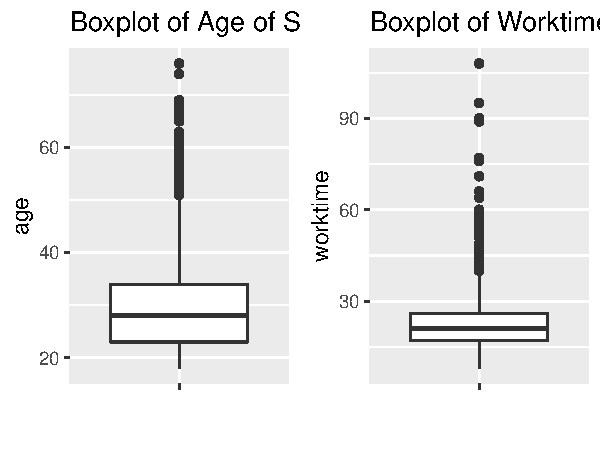
\includegraphics{hw3_sp2022_files/figure-latex/unnamed-chunk-10-1.pdf}

\begin{Shaded}
\begin{Highlighting}[]
\FunctionTok{plot}\NormalTok{(}\FunctionTok{lm}\NormalTok{(mpg }\SpecialCharTok{\textasciitilde{}}\NormalTok{ weight, }\AttributeTok{data=}\NormalTok{Auto), }\DecValTok{1}\NormalTok{)}
\end{Highlighting}
\end{Shaded}

\includegraphics{hw3_sp2022_files/figure-latex/unnamed-chunk-10-2.pdf}

From this graph, we can see that the GPM regression with weight is a
better option. For GPM, the residuals are spread randomly around the 0
line. This suggests that the assumption that the relationship is linear
is reasonable for this model. The graph also suggests that the variances
of the error term are normal, i.e., we have Homoscedasticity.

\begin{Shaded}
\begin{Highlighting}[]
\FunctionTok{plot}\NormalTok{(}\FunctionTok{lm}\NormalTok{(gpm }\SpecialCharTok{\textasciitilde{}}\NormalTok{ weight, }\AttributeTok{data=}\NormalTok{Auto), }\DecValTok{2}\NormalTok{)}
\end{Highlighting}
\end{Shaded}

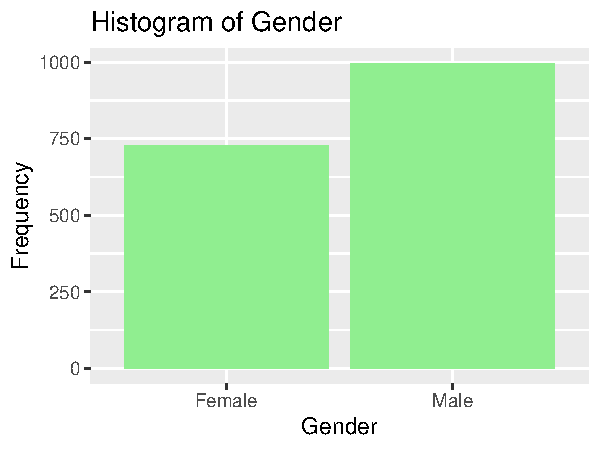
\includegraphics{hw3_sp2022_files/figure-latex/unnamed-chunk-11-1.pdf}
We also have the normality assumption met for GPM.

Thus for our linear model, we will select to use GPM as the assumptions
are all met with GPM.

Another reason to not use MPG, is MPG will tell you the range of the
car's gas tank, this means that it could vary significantly between cars
as all tank sizes are not the same. GPM is useful when you are comparing
different cars as it allows you to better captures the fuel consumption
of the car. By using GPM, you can tell how much gas you will need to use
for a certain length of driving. This allows for efficiency in comparing
different cars to one uniform distance.

Before we begin the model, we are going to look at whether or not we
should use cylinders as a numeric or a factor. Clearly origin should be
a factor as it is three specific values that represent a categorical
variable, however, cylinders in numeric in nature.

First let's only include the variables that make sense for the
regression, i.e., we will not be including names for the regression and
we removed MPG as we will be using GPM.

\begin{Shaded}
\begin{Highlighting}[]
\NormalTok{names.exclude }\OtherTok{\textless{}{-}} \FunctionTok{names}\NormalTok{(Auto) }\SpecialCharTok{\%in\%} \FunctionTok{c}\NormalTok{(}\StringTok{"name"}\NormalTok{, }\StringTok{"mpg"}\NormalTok{)}
\NormalTok{Auto2 }\OtherTok{\textless{}{-}}\NormalTok{ Auto[}\SpecialCharTok{!}\NormalTok{names.exclude]  }
\FunctionTok{names}\NormalTok{(Auto2)    }\CommentTok{\#str(data2)   table(data2$Transmission)}
\end{Highlighting}
\end{Shaded}

\begin{verbatim}
## [1] "cylinders"    "displacement" "horsepower"   "weight"       "acceleration"
## [6] "year"         "origin"       "gpm"
\end{verbatim}

We will make origin into a factor here.

\begin{Shaded}
\begin{Highlighting}[]
\NormalTok{Auto2}\SpecialCharTok{$}\NormalTok{origin }\OtherTok{\textless{}{-}} \FunctionTok{as.factor}\NormalTok{(Auto2}\SpecialCharTok{$}\NormalTok{origin)}
\FunctionTok{str}\NormalTok{(Auto2}\SpecialCharTok{$}\NormalTok{origin)}
\end{Highlighting}
\end{Shaded}

\begin{verbatim}
##  Factor w/ 3 levels "1","2","3": 1 1 1 1 1 1 1 1 1 1 ...
\end{verbatim}

Now we will compare the regression for cylinder as a numeric and
cylinder as a factor.

\begin{Shaded}
\begin{Highlighting}[]
\NormalTok{fit.cyl.number }\OtherTok{\textless{}{-}} \FunctionTok{lm}\NormalTok{(gpm}\SpecialCharTok{\textasciitilde{}}\NormalTok{. , Auto2)}
\end{Highlighting}
\end{Shaded}

\begin{Shaded}
\begin{Highlighting}[]
\NormalTok{Auto2}\SpecialCharTok{$}\NormalTok{cylinders }\OtherTok{\textless{}{-}} \FunctionTok{as.factor}\NormalTok{(Auto2}\SpecialCharTok{$}\NormalTok{cylinders)}
\NormalTok{fit.cyl.factor }\OtherTok{\textless{}{-}} \FunctionTok{lm}\NormalTok{(gpm}\SpecialCharTok{\textasciitilde{}}\NormalTok{. , Auto2)}
\FunctionTok{anova}\NormalTok{(fit.cyl.number, fit.cyl.factor)}
\end{Highlighting}
\end{Shaded}

\begin{verbatim}
## Analysis of Variance Table
## 
## Model 1: gpm ~ cylinders + displacement + horsepower + weight + acceleration + 
##     year + origin
## Model 2: gpm ~ cylinders + displacement + horsepower + weight + acceleration + 
##     year + origin
##   Res.Df    RSS Df Sum of Sq    F Pr(>F)   
## 1    383 0.0123                            
## 2    380 0.0117  3  0.000511 5.51  0.001 **
## ---
## Signif. codes:  0 '***' 0.001 '**' 0.01 '*' 0.05 '.' 0.1 ' ' 1
\end{verbatim}

Although the variable \texttt{cylinders} is numeric in nature, it is
highly, non linear. This means that it is more valuable to consider this
variable as a factor instead of it's numeric value. Further looking at
the analysis of variance for the two variables, with a null hypothesis
that the two different fits are the same, we reject the null hypothesis
at a level of 0.01, as the p-value is 0.001. Thus, we get that the two
fits are significantly different and from our analysis, it would be
beneficial to use cylinders as a factor.

\begin{enumerate}
\def\labelenumi{\arabic{enumi})}
\setcounter{enumi}{1}
\tightlist
\item
  Describe the final model and its accuracy. Include diagnostic plots
  with particular focus on the model residuals.
\end{enumerate}

\begin{itemize}
\tightlist
\item
  Summarize the effects found.
\item
  Predict the \texttt{mpg} of a car that is: built in 1983, in the US,
  red, 180 inches long, 8 cylinders, 350 displacement, 260 as
  horsepower, and weighs 4,000 pounds. Give a 95\% CI.
\item
  Any suggestions as to how to improve the quality of the study?
\end{itemize}

\hypertarget{case-study-2-covid}{%
\section{Case study 2: COVID}\label{case-study-2-covid}}

See covid\_case\_study.Rmd.

\end{document}
